\chapter{Project Closing and Lessons Learned}

\section{Success Criteria Satisfaction}

All the specified success criteria for the Recreation and Wellness Intranet Project were satisfied:

\begin{itemize}
    \item \textbf{Scope:} The project developed a web-based application that records employee activity, provides rewards, and enables staff members to sign up for company-sponsored classes, leisure activities, and health-management programs.
    \item \textbf{Time:} In consistent with the initial plan, the project was finished in six months.
    \item \textbf{Cost:} The project stayed within the original budget of \$200,000.
    \item \textbf{Self-sufficiency:} The project achieved self-sufficiency within one year of implementation, meaning that the revenue generated from the incentive program is now covering the cost of maintaining and operating the application.
\end{itemize}

\textbf{Critical lessons learned:} Managing the Recreation and Wellness Intranet Project taught the project team some important lessons:

\begin{itemize}
    \item Be proactive in managing stakeholder expectations. It is important to keep stakeholders informed of the project progress and any changes to the plan, even if they are not directly involved in the day-to-day work. This helps to avoid surprises and ensure that everyone is on the same page.
    \item Use a variety of communication channels to reach stakeholders. Not everyone prefers the same way to communicate. Some stakeholders may prefer email, while others may prefer face-to-face meetings or phone calls. It is important to use a variety of communication channels to ensure that everyone can stay informed.
    \item Create a detailed project plan and budget. This will help to keep the project on track and avoid overspending. In order to ensure that the project plan and budget are still valid, it is also crucial to keep monitoring them.
    \item Conduct thorough testing of the application before launch. This will help to identify and fix any bugs or usability issues. It is also important to get feedback from users before launching the application to ensure that it meets their needs.
    \item Track and measure the success of the application. This will help to identify what is working well and what needs to be improved. It is also important to share the success of the application with stakeholders to show them the value of the project.
\end{itemize}

\section{Examples of What Went Right and Wrong}

\subsection{Examples of What Went Right}

\begin{itemize}
    \item Effective collaboration with stakeholders: The project team established a robust rapport with stakeholders, facilitating the comprehensive definition of requirements. This engagement ensured that the final product seamlessly aligned with users' needs. For instance, conducting an employee survey provided invaluable insights into recreational programs, health-management classes, and incentives.
    \item Methodical project management: The team's adherence to a structured project management methodology proved instrumental in project success. The utilization of tools like Gantt charts for scheduling and risk registers for risk assessment and mitigation ensured that the project adhered to timelines and goals.
    \item Rigorous application testing: Prior to the official launch, the project team rigorously tested the application, uncovering and rectifying bugs and usability concerns. User acceptance testing, involving a select group of employees, was conducted to gather feedback and refine the application before its organization-wide deployment.
    \item Proactive application promotion: To guarantee the application's success, the team actively promoted it among employees. Creating a dedicated website, establishing a social media presence, and sending out informative email announcements encouraged its adoption.
\end{itemize}

\subsection{Examples of What Went Wrong}

\begin{itemize}
    \item One challenge encountered was underestimating the time required for application development and launch. For instance, the team miscalculated the development duration for the tracking system, necessitating last-minute efforts, and causing stress to meet the deadline.
    \item Lack of familiarity with new tools caused delays and required additional training, which incurred extra costs and extended project timelines
\end{itemize}

\section{What We Might Change for the Upcoming Project}

We would approach the next project differently, having learned from our experience with the Recreation and Wellness Intranet Project:

\begin{itemize}
    \item Keep stakeholders informed about the team's composition and any potential hazards early and frequently. Expectations will be better managed and unpleasant surprises will be avoided. Stakeholders would be updated on project progress and any modifications to the plan through frequent status meetings. Additionally, we would give out frequent email updates.
    \item By determining the maximum buffer period, we can create a project schedule and budget that are more specific. By doing this, delays and wasteful money would be reduced.
    \item Identify the main players on the team and create backup plans for each position. This can need instructing more team members on the relevant skills, or it might entail using consultants to cover for absent team members.
\end{itemize}

We believe that with the identified solution for multiple issues based on this project, we can ensure that future projects are successful.

\section{Additional Thoughts}

Throughout our project's duration, we saw a notable level of accomplishment, with teamwork and structured organization taking center stage. A cornerstone of this achievement was our adoption of collaborative tech tools. Primarily, GitHub emerged as our chief project coordination platform, harmoniously working alongside Microsoft 365's comprehensive toolkit, with a special nod to Microsoft Project. Tasks were systematically listed on a GitHub project board, allowing team members to pick and assign tasks based on consensus during team discussions. They could also update their statuses and benchmark their pace against predetermined deadlines. Many assignments were prepared using cloud versions of Microsoft Word, Excel, and Project, and completed tasks were archived in a shared folder on Microsoft OneDrive. These platforms made it possible to assign tasks and monitor progress, which encouraged members to take responsibility for their actions. The real-time updating feature and the capacity for simultaneous collaborative efforts minimized potential lags in our timeline, leading to a smooth, timely, and harmonious working environment.

\begin{figure}[ht]
    \centering
    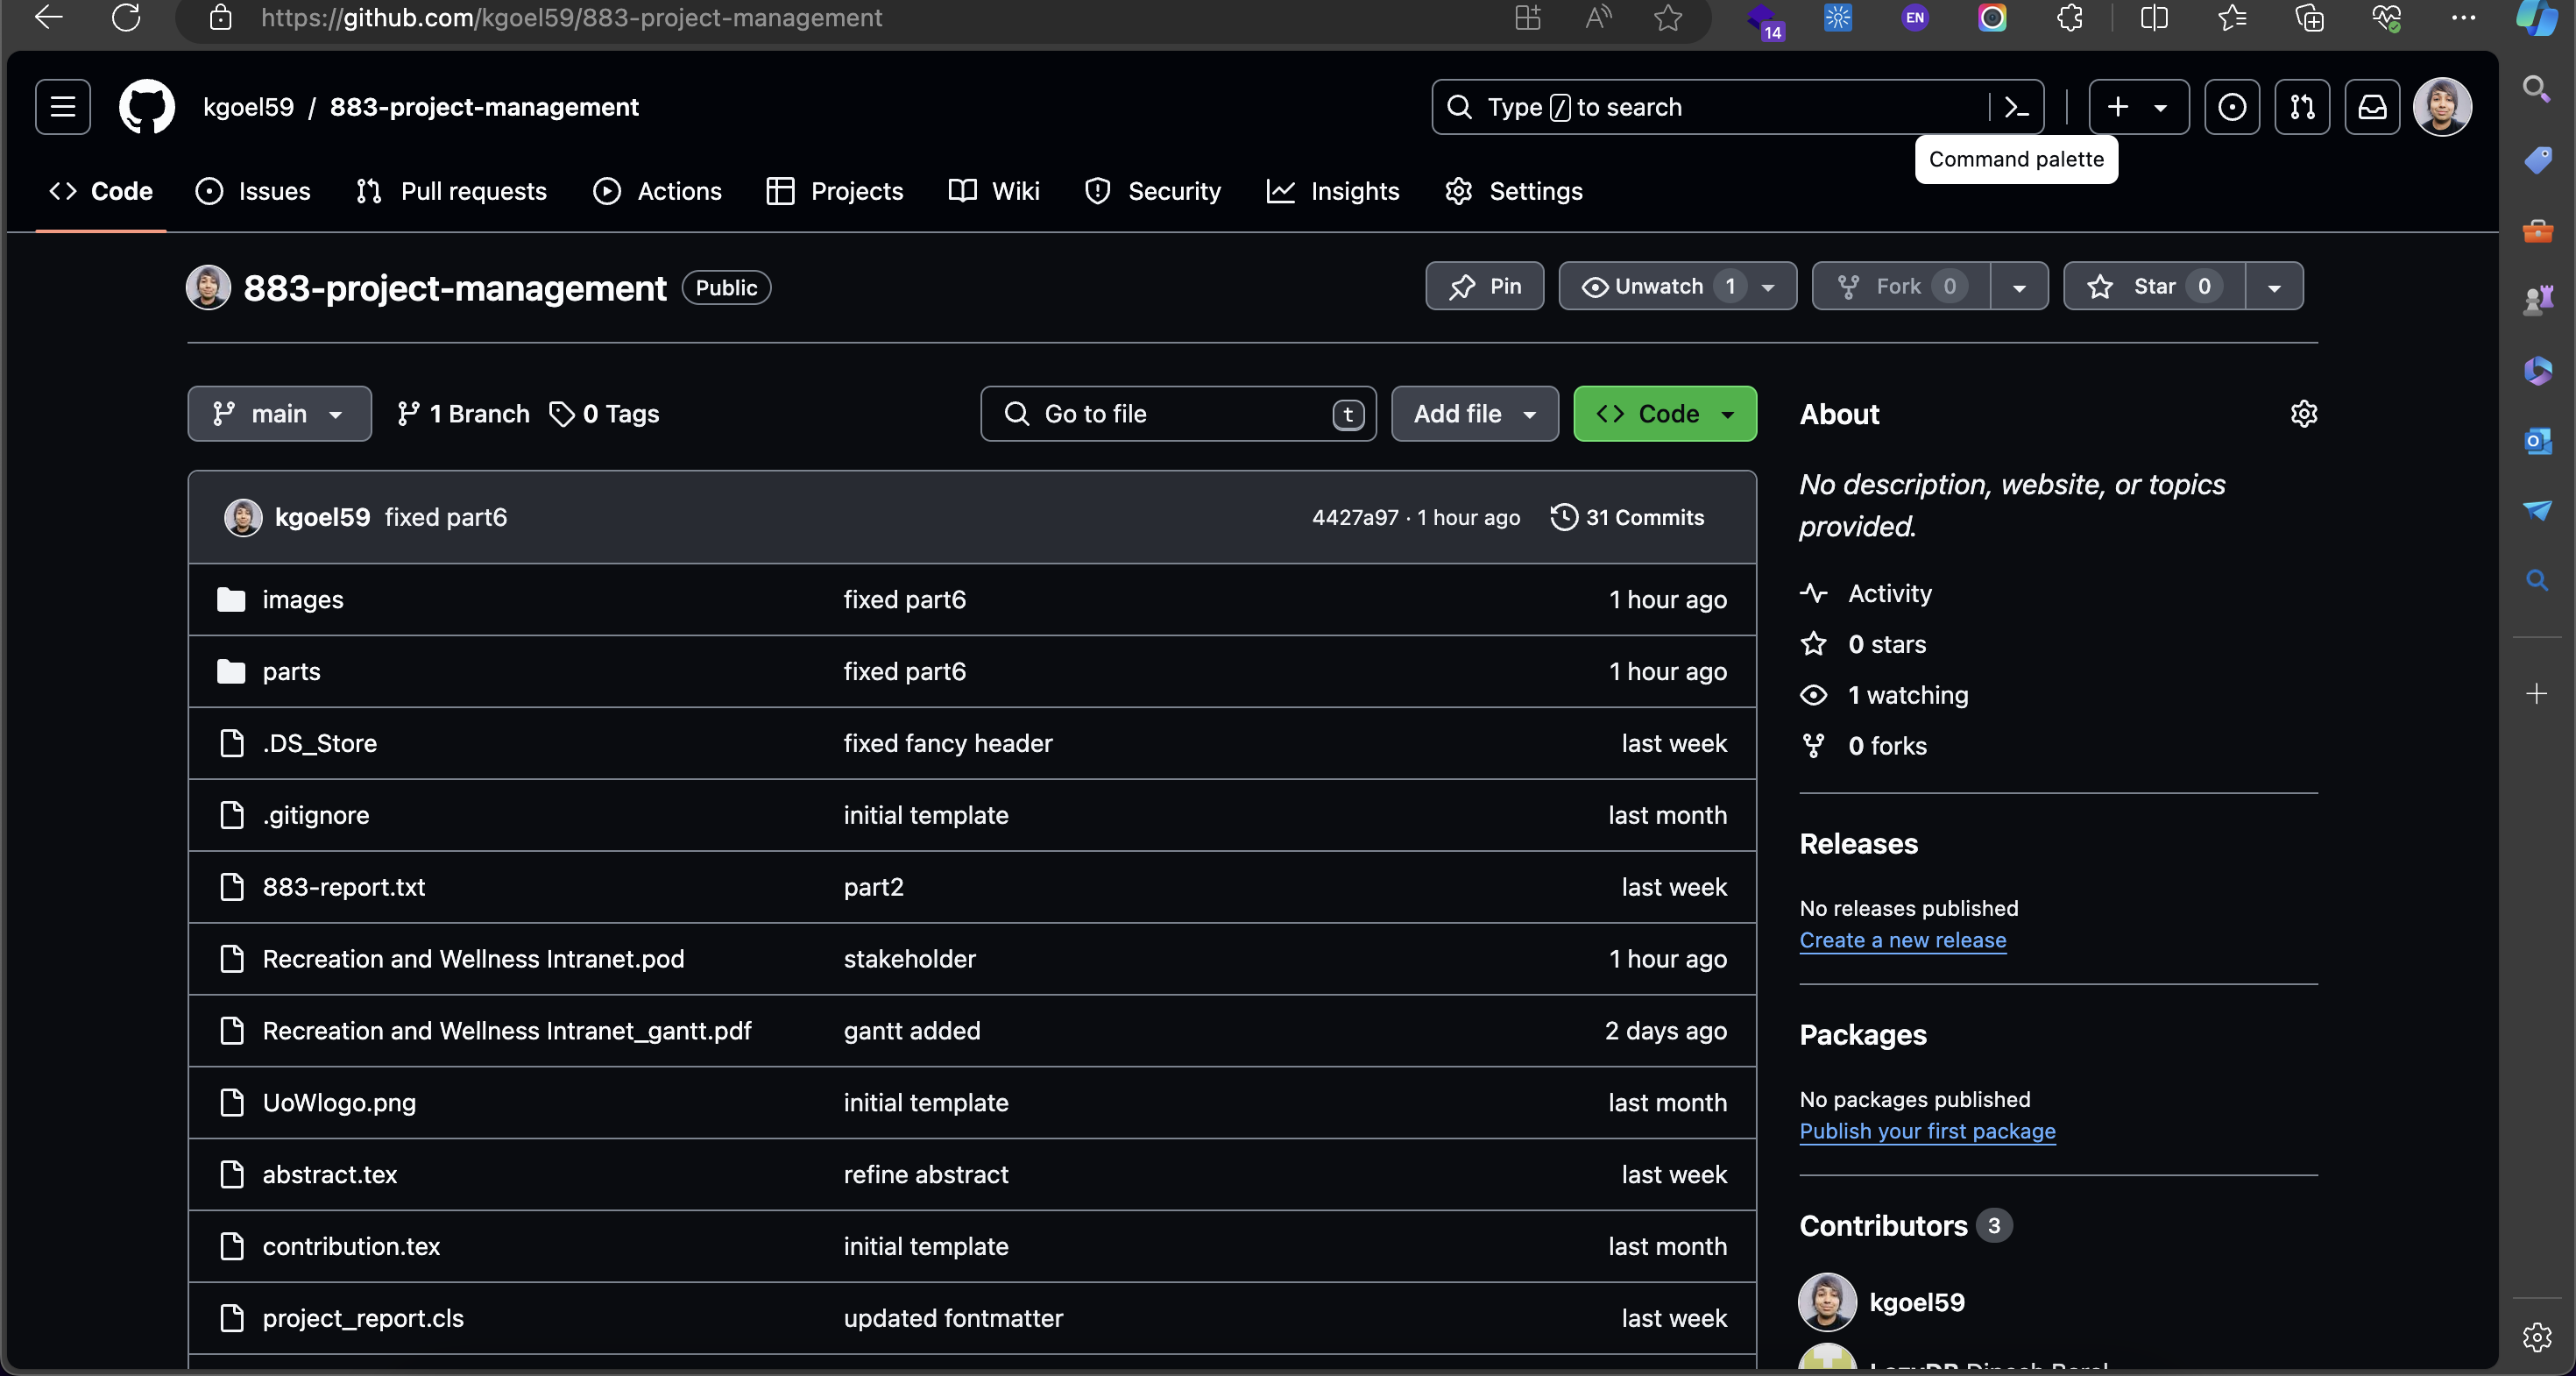
\includegraphics[width=0.8\textwidth]{images/github.png}
    \caption{Using GitHub in Project Management}
    \label{fig:github}
\end{figure}


\FloatBarrier
\newpage